\documentclass{beamer}
\usepackage{fontspec}
\usepackage{listings}
\usepackage{xcolor}
\usepackage{booktabs}
\usepackage{amsmath}
\usepackage{amssymb}
\usepackage{array}
\usepackage{colortbl}
\usepackage{tikz}
\usetikzlibrary{positioning, shapes.geometric, calc}

\setmainfont{Noto Sans CJK KR}[BoldFont={Noto Sans CJK KR Bold}]
\setsansfont{Noto Sans CJK KR}[BoldFont={Noto Sans CJK KR Bold}]
\setmonofont{DejaVu Sans Mono}

\usetheme{Madrid}
\usecolortheme{default}

\definecolor{navyblue}{HTML}{1E3A5F}
\definecolor{accentblue}{HTML}{3B82F6}
\definecolor{lightblue}{HTML}{DBEAFE}
\definecolor{codegreen}{HTML}{059669}
\definecolor{lightgreen}{HTML}{D1FAE5}
\definecolor{codered}{HTML}{DC2626}
\definecolor{lightred}{HTML}{FEE2E2}
\definecolor{amber}{HTML}{B45309}
\definecolor{lightamber}{HTML}{FEF3C7}
\definecolor{codebg}{HTML}{1E293B}
\definecolor{codefg}{HTML}{E2E8F0}
\definecolor{slategray}{HTML}{475569}
\definecolor{purple}{HTML}{7C3AED}
\definecolor{lightpurple}{HTML}{EDE9FE}

\setbeamercolor{palette primary}{bg=navyblue, fg=white}
\setbeamercolor{palette secondary}{bg=navyblue!80, fg=white}
\setbeamercolor{palette tertiary}{bg=navyblue!60, fg=white}
\setbeamercolor{palette quaternary}{bg=navyblue, fg=white}
\setbeamercolor{structure}{fg=navyblue}
\setbeamercolor{frametitle}{bg=navyblue, fg=white}
\setbeamercolor{title}{bg=navyblue!95!black, fg=white}
\setbeamercolor{block title}{bg=navyblue, fg=white}
\setbeamercolor{block body}{bg=lightblue!50, fg=black}
\setbeamercolor{block title alerted}{bg=codered, fg=white}
\setbeamercolor{block body alerted}{bg=lightred!60, fg=black}
\setbeamercolor{block title example}{bg=codegreen, fg=white}
\setbeamercolor{block body example}{bg=lightgreen!60, fg=black}

\lstdefinestyle{cpp}{
    language=C++,
    basicstyle=\ttfamily\scriptsize\color{codefg},
    keywordstyle=\color{accentblue}\bfseries,
    commentstyle=\color{slategray}\itshape,
    stringstyle=\color{lightgreen},
    showstringspaces=false,
    backgroundcolor=\color{codebg},
    frame=single, framerule=0.5pt, rulecolor=\color{slategray},
    breaklines=true, keepspaces=true, columns=flexible,
    xleftmargin=4pt, xrightmargin=4pt,
}

\title{Discrete Mathematics}
\subtitle{Week 2 -- Sets, Functions \& Matrices}
\author{JeYoung Park}
\institute{SeoulTech CS\&CE}
\date{2026-03-26}

\begin{document}

% ══════════════════════════════════════════════════════════
% TITLE
% ══════════════════════════════════════════════════════════
\begin{frame}
    \titlepage
\end{frame}

% ══════════════════════════════════════════════════════════
% OUTLINE
% ══════════════════════════════════════════════════════════
\begin{frame}{Today's Roadmap}
    \small
    \begin{columns}[T]
        \column{0.48\textwidth}
        \textbf{Part 1: Sets}
        \vspace{0.1cm}

        \footnotesize
        \begin{enumerate}\setlength\itemsep{0.15em}
            \item Set -- Definition \& Notation
            \item Subset, Power Set
            \item Cartesian Product
            \item Set Operations \& Identities
            \item Bit Representation \& C++
            \item Multiset, Countability
        \end{enumerate}

        \column{0.48\textwidth}
        \textbf{Part 2: Functions \& Matrices}
        \vspace{0.1cm}

        \footnotesize
        \begin{enumerate}\setlength\itemsep{0.15em}
            \setcounter{enumi}{6}
            \item Functions
            \item Matrix -- Definition \& Operations
            \item Boolean Matrix
            \item Practice Problems
        \end{enumerate}
    \end{columns}

    \vspace{0.3cm}
    \begin{alertblock}{CS Motivation}
        \footnotesize
        \textbf{Set} = type system, DB, bitmask\\
        \textbf{Matrix} = graph, relation, network
    \end{alertblock}
\end{frame}

% ══════════════════════════════════════════════════════════
% BRIDGE FROM WEEK 1
% ══════════════════════════════════════════════════════════
\begin{frame}[t,shrink=5]{Week 1 Review \& Week 2 Bridge}
    \small
    \vspace{0.1cm}
    \begin{block}{Last Week}
        \footnotesize Proposition 과 논리 연산자로 \textbf{참/거짓을 판별}하는 언어를 배웠습니다.\\
        $p \land q, \quad p \lor q, \quad \neg p, \quad p \rightarrow q$
    \end{block}

    \vspace{0.15cm}
    \textbf{This Week: Proposition $\to$ Set}

    \begin{center}
    \footnotesize
    \renewcommand{\arraystretch}{1.3}
    \begin{tabular}{ccc}
        \toprule
        \textbf{Week 1 (Logic)} & & \textbf{Week 2 (Set)} \\
        \midrule
        $p \land q$ & $\longleftrightarrow$ & $A \cap B$ \\
        $p \lor q$  & $\longleftrightarrow$ & $A \cup B$ \\
        $\neg p$    & $\longleftrightarrow$ & $\overline{A}$ (complement) \\
        $p \rightarrow q$ & $\longleftrightarrow$ & $A \subseteq B$ \\
        \bottomrule
    \end{tabular}
    \renewcommand{\arraystretch}{1}
    \end{center}

    \vspace{0.1cm}
    \begin{exampleblock}{Why Sets Matter in CS}
        \footnotesize
        C++의 \texttt{int}, \texttt{bool}, \texttt{char} 같은 \textbf{데이터 타입}은 집합 위에 정의됩니다.\\
        예: \texttt{boolean}은 집합 $\{0, 1\}$에 \texttt{AND}, \texttt{OR}, \texttt{NOT} 연산을 붙인 것입니다.\\[2pt]
        \textbf{Set = 수학적 데이터 구조의 기반}, \textbf{Matrix = 관계를 숫자로 표현하는 언어}
    \end{exampleblock}
\end{frame}

% ══════════════════════════════════════════════════════════
% PART 1: SETS
% ══════════════════════════════════════════════════════════

% ══ SET DEFINITION ═══════════════════════════════════════
\begin{frame}[t,shrink=3]{Set -- Definition \& Notation}
    \small
    \vspace{0.1cm}
    \begin{block}{Definition}
        \textbf{Set}은 순서 상관 없이 모인 \textbf{서로 구별되는 객체(elements / members)}의 모음입니다.
    \end{block}

    \vspace{0.1cm}
    \begin{columns}[T]
        \column{0.48\textwidth}
        \textbf{Notation}
        \vspace{0.05cm}

        \footnotesize
        \begin{itemize}\setlength\itemsep{0.2em}
            \item \textbf{Roster method}: $A = \{1, 2, 3, 4\}$
            \item \textbf{Set-builder notation}:\\
                  $B = \{x \mid x \text{ has property } P\}$\\
                  ``the set of all $x$ s.t.\ $x$ has property $P$''\\
                  e.g.\ $\{x \mid x \text{ is a positive even}\} = \{2,4,6,\ldots\}$
            \item $2 \in A$ \quad (element of)
            \item $5 \notin A$ \quad (not element of)
        \end{itemize}

        \column{0.48\textwidth}
        \textbf{Well-known Sets}
        \vspace{0.05cm}

        \footnotesize
        \begin{itemize}\setlength\itemsep{0.2em}
            \item $\emptyset$ \quad empty set
            \item $\mathbb{N}$ \quad $\{0, 1, 2, \ldots\}$
            \item $\mathbb{Z}$ \quad $\{\ldots, -1, 0, 1, \ldots\}$
            \item $\mathbb{Q}$ \quad rationals
            \item $\mathbb{R}$ \quad reals
            \item $U$ \quad universal set
        \end{itemize}
    \end{columns}

    \vspace{0.15cm}
    \begin{alertblock}{REMARK}
        \scriptsize
        \textbf{Order does not matter:} $\{1, 2, 3\} = \{3, 1, 2\}$ \qquad
        \textbf{No duplicates:} $\{1, 1, 2\} = \{1, 2\}$\\[2pt]
        \textbf{Equality:} $A = B \;\Leftrightarrow\; \forall x\,(x \in A \leftrightarrow x \in B)$
    \end{alertblock}
\end{frame}

% ══ DATATYPE = SET + OPERATIONS ══════════════════════════
\begin{frame}[t]{Datatype = Set + Operations}
    \small
    \vspace{0.1cm}
    \begin{block}{Definition}
        \footnotesize
        \textbf{Datatype (Type)} = 집합의 이름 + 그 집합 위에 정의된 연산(operation)들
    \end{block}

    \vspace{0.15cm}
    \footnotesize
    \renewcommand{\arraystretch}{1.4}
    \begin{tabular}{lll}
        \toprule
        \textbf{C++ Type} & \textbf{Underlying Set} & \textbf{Operations} \\
        \midrule
        \texttt{bool} & $\{0, 1\}$ (\texttt{false}, \texttt{true}) & \texttt{\&\&}, \texttt{||}, \texttt{!} \\
        \texttt{char} & $\{0, 1, \ldots, 255\}$ & comparison, arithmetic \\
        \texttt{int} & $\{-2^{31}, \ldots, 2^{31}{-}1\}$ & \texttt{+}, \texttt{-}, \texttt{*}, \texttt{/}, \texttt{\%} \\
        \texttt{unsigned int} & $\{0, 1, \ldots, 2^{32}{-}1\}$ & \texttt{+}, \texttt{-}, \texttt{*}, bitwise ops \\
        \bottomrule
    \end{tabular}
    \renewcommand{\arraystretch}{1}

    \vspace{0.2cm}
    \begin{exampleblock}{Why This Matters}
        \footnotesize
        Type system이 집합론에 기반하므로,\\
        후에 \textbf{type safety}, \textbf{overflow}, \textbf{casting}의 동작 원리 또한 Set+operations 에 의존 합니다.
    \end{exampleblock}
\end{frame}

% ══ SUBSET & PROPER SUBSET ═══════════════════════════════
\begin{frame}[t,shrink=3]{Subset vs Proper Subset}
    \small
    \vspace{0.1cm}
    \begin{columns}[T]
        \column{0.48\textwidth}
        \begin{block}{Subset $A \subseteq B$}
            \footnotesize
            $A$의 \textbf{모든} 원소가 $B$에도 포함\\[4pt]
            $A \subseteq B \;\Leftrightarrow\; \forall x\,(x \in A \rightarrow x \in B)$
        \end{block}

        \vspace{0.1cm}
        \begin{block}{Proper Subset $A \subset B$}
            \footnotesize
            $A$는 $B$의 부분집합이지만 $A \neq B$\\[4pt]
            $A \subset B \;\Leftrightarrow\; (A \subseteq B) \land (A \neq B)$\\[4pt]
            즉, $\forall x(x \in A \to x \in B) \;\land\; \exists x(x \in B \land x \notin A)$\\[4pt]
            $B$에는 있지만 $A$에는 없는 원소가 \textbf{적어도 하나} 존재
        \end{block}

        \column{0.48\textwidth}
        \begin{exampleblock}{Example}
            \footnotesize
            $A = \{1, 2\}$, \; $B = \{1, 2, 3\}$\\[4pt]
            $A \subseteq B$ \quad \checkmark \quad (1,2 모두 $B$에 있음)\\
            $A \subset B$ \quad \checkmark \quad (3이 $B$에만 있음)\\
            $B \subseteq A$ \quad $\times$ \quad ($3 \in B$ 이지만 $3 \notin A$)\\[6pt]
            $C = \{1, 2, 3\}$\\
            $B \subseteq C$ \quad \checkmark\\
            $B \subset C$ \quad $\times$ \quad ($B = C$)
        \end{exampleblock}

        \vspace{0.1cm}
        \begin{alertblock}{REMARK}
            \scriptsize
            모든 집합 $S$에 대해:\\
            $\emptyset \subseteq S$ \quad (공집합은 모든 집합의 부분집합)\\
            $S \subseteq S$ \quad (자기 자신도 부분집합)
        \end{alertblock}
    \end{columns}
\end{frame}

% ══ CARDINALITY & POWER SET ══════════════════════════════
\begin{frame}[t,shrink=3]{Cardinality \& Power Set}
    \small
    \vspace{0.1cm}
    \begin{columns}[T]
        \column{0.48\textwidth}
        \begin{block}{Cardinality $|A|$}
            \footnotesize
            집합 $A$의 원소 수\\[4pt]
            $A = \{a, b, c\}$ $\Rightarrow$ $|A| = 3$\\
            $|\emptyset| = 0$\\[6pt]
            \textbf{Finite set}: $|A|$가 자연수\\
            \textbf{Infinite set}: A set is said to be\\
            infinite if it is not finite\\
            e.g.\ $|\mathbb{N}| = \infty$, \; $|\mathbb{Z}| = \infty$
        \end{block}

        \vspace{0.1cm}
        \begin{alertblock}{\scriptsize In C++}
            \scriptsize \texttt{std::set<int> s;}\\
            \texttt{s.size()} $= |S|$ (cardinality)\\
            \texttt{s.empty()} $\leftrightarrow$ $S = \emptyset$
        \end{alertblock}

        \column{0.48\textwidth}
        \begin{block}{Power Set $\mathcal{P}(A)$}
            \footnotesize
            $\mathcal{P}(A)$ : $A$의 \textbf{모든 부분집합}의 집합\\[4pt]
            $|A| = n \;\Rightarrow\; |\mathcal{P}(A)| = 2^n$
        \end{block}

        \vspace{0.1cm}
        \begin{exampleblock}{Example: $A = \{a, b, c\}$}
            \footnotesize
            $\mathcal{P}(A) = \bigl\{\emptyset,\; \{a\},\; \{b\},\; \{c\},$\\
            $\phantom{\mathcal{P}(A) = \bigl\{}\{a,b\},\; \{a,c\},\; \{b,c\},\; \{a,b,c\}\bigr\}$\\[4pt]
            $|\mathcal{P}(A)| = 2^3 = 8$
        \end{exampleblock}

        \vspace{0.1cm}
        \begin{alertblock}{\scriptsize Why $2^n$?}
            \scriptsize 각 원소에 대해 ``포함 / 미포함'' 2가지 선택\\
            $n$개 원소 $\to$ $\underbrace{2 \times 2 \times \cdots \times 2}_{n} = 2^n$\\
            $=$ \textbf{bitmask}로 열거 가능 ($n$-bit integer)
        \end{alertblock}
    \end{columns}
\end{frame}

% ══ CARTESIAN PRODUCT ════════════════════════════════════
\begin{frame}[t,shrink=3]{Cartesian Product}
    \small
    \vspace{0.1cm}
    \begin{block}{Definition}
        $A \times B = \{(a, b) \mid a \in A \;\land\; b \in B\}$\\[4pt]
        \footnotesize $A$와 $B$의 원소로 만들 수 있는 \textbf{모든 ordered pair의 집합}
    \end{block}

    \vspace{0.1cm}
    \begin{columns}[T]
        \column{0.48\textwidth}
        \begin{exampleblock}{Example}
            \footnotesize
            $A = \{1, 2\}$, $B = \{a, b, c\}$\\[4pt]
            $A \times B = \{(1,a),(1,b),(1,c),$\\
            $\phantom{A \times B = \{}(2,a),(2,b),(2,c)\}$\\[4pt]
            $|A \times B| = |A| \cdot |B| = 6$
        \end{exampleblock}

        \vspace{0.08cm}
        \begin{alertblock}{REMARK}
            \scriptsize
            $A \times B \neq B \times A$ \; (순서쌍은 순서가 중요!)\\
            $(A \times B) \times C \neq A \times B \times C$\\
            ($((1,2),3)$ vs $(1,2,3)$ -- 구조가 다름)\\[2pt]
            Exception: $A = \emptyset$ or $B = \emptyset$ or $A = B$
        \end{alertblock}

        \column{0.48\textwidth}
        \begin{block}{CS Applications}
            \footnotesize
            \textbf{Relation}: $R \subseteq A \times B$\\[4pt]
            e.g.\ Student--Course enrollment\\
            $(\text{Alice},\; \text{DiscreteMath}) \in R$\\[6pt]
            \textbf{DB table}: each row = tuple\\
            \textbf{Graph edge}: $(u, v) \in E \subseteq V \times V$
        \end{block}

        \vspace{0.08cm}
        \begin{exampleblock}{\scriptsize In C++}
            \scriptsize
            \texttt{pair<int,char> p = \{1,'a'\};}\\
            \texttt{// p.first=1, p.second='a'}\\
            \texttt{// (1,'a')} $\in$ \texttt{int} $\times$ \texttt{char}
        \end{exampleblock}
    \end{columns}
\end{frame}

% ══ SET OPERATIONS ═══════════════════════════════════════
\begin{frame}[t,shrink=5]{Set Operations}
    \small
    \vspace{0.1cm}
    \begin{columns}[T]
        \column{0.52\textwidth}
        \footnotesize
        \renewcommand{\arraystretch}{1.35}
        \begin{tabular}{lll}
            \toprule
            \textbf{Operation} & \textbf{Symbol} & \textbf{Definition} \\
            \midrule
            Union & $A \cup B$ & $\{x \mid x \in A \lor x \in B\}$ \\
            Intersection & $A \cap B$ & $\{x \mid x \in A \land x \in B\}$ \\
            Difference & $A - B$ & $\{x \mid x \in A \land x \notin B\}$ \\
            Complement & $\overline{A}$ & $\{x \in U \mid x \notin A\}$ \\
            Sym.\ Diff. & $A \oplus B$ & $(A - B) \cup (B - A)$ \\
            \bottomrule
        \end{tabular}
        \renewcommand{\arraystretch}{1}

        \vspace{0.1cm}
        \begin{exampleblock}{Example}
            \scriptsize
            $A = \{1,2,3,4\}$, $B = \{3,4,5,6\}$, $U = \{1,\ldots,6\}$\\[3pt]
            $A \cup B = \{1,2,3,4,5,6\}$ \quad
            $A \cap B = \{3,4\}$\\
            $A - B = \{1,2\}$ \quad
            $\overline{A} = \{5,6\}$\\
            $A \oplus B = \{1,2,5,6\}$
        \end{exampleblock}

        \column{0.44\textwidth}
        \textbf{Venn Diagram}
        \vspace{0.05cm}

        \centering
        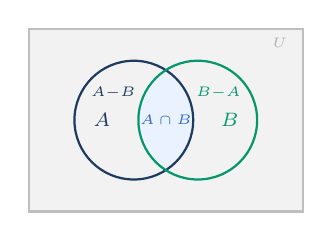
\begin{tikzpicture}[scale=0.58]
            \fill[gray!10] (-3,-2) rectangle (3,2);
            \draw[gray!50, thick] (-3,-2) rectangle (3,2);
            \node[gray!60, font=\tiny] at (2.5,1.7) {$U$};
            \begin{scope}
                \clip (-0.7,0) circle (1.3cm);
                \fill[lightblue!60] (0.7,0) circle (1.3cm);
            \end{scope}
            \draw[navyblue, thick] (-0.7,0) circle (1.3cm);
            \draw[codegreen, thick] (0.7,0) circle (1.3cm);
            \node[navyblue, font=\bfseries\scriptsize] at (-1.4,0) {$A$};
            \node[codegreen, font=\bfseries\scriptsize] at (1.4,0) {$B$};
            \node[accentblue!80!black, font=\tiny] at (0,0) {$A \cap B$};
            \node[navyblue, font=\tiny] at (-1.15,0.6) {$A{-}B$};
            \node[codegreen, font=\tiny] at (1.15,0.6) {$B{-}A$};
        \end{tikzpicture}

        \vspace{0.1cm}
        \begin{block}{\scriptsize Logic $\leftrightarrow$ Set}
            \scriptsize
            $A \cup B \;\leftrightarrow\; p \lor q$ \qquad
            $A \cap B \;\leftrightarrow\; p \land q$\\
            $\overline{A} \;\leftrightarrow\; \neg p$ \qquad\quad
            $A \oplus B \;\leftrightarrow\; p \oplus q$
        \end{block}
    \end{columns}
\end{frame}

% ══ SET IDENTITIES ═══════════════════════════════════════
\begin{frame}[t,shrink=8]{Set Identities}
    \small
    \vspace{0.05cm}
    \begin{alertblock}{REMARK}
        \scriptsize Week 1의 \textbf{논리 동치 법칙}과 완전히 같은 구조! $\;\land \leftrightarrow \cap$, $\;\lor \leftrightarrow \cup$, $\;\neg \leftrightarrow \overline{\phantom{A}}$ 로 치환하면 됩니다.
    \end{alertblock}

    \vspace{0.05cm}
    \begin{center}
    \scriptsize
    \renewcommand{\arraystretch}{1.3}
    \begin{tabular}{lll}
        \toprule
        \textbf{Set Identity} & \textbf{Logical Equiv.} & \textbf{Name} \\
        \midrule
        $A \cap U = A$, \; $A \cup \emptyset = A$ & $p \land \mathbf{T} \equiv p$, \; $p \lor \mathbf{F} \equiv p$ & Identity \\
        $A \cup U = U$, \; $A \cap \emptyset = \emptyset$ & $p \lor \mathbf{T} \equiv \mathbf{T}$, \; $p \land \mathbf{F} \equiv \mathbf{F}$ & Domination \\
        $A \cup A = A$, \; $A \cap A = A$ & $p \lor p \equiv p$, \; $p \land p \equiv p$ & Idempotent \\
        $\overline{(\overline{A})} = A$ & $\neg\neg p \equiv p$ & Double Complement \\
        $A \cup B = B \cup A$, \; $A \cap B = B \cap A$ & Commutative & Commutative \\
        $(A \cup B) \cup C = A \cup (B \cup C)$ & Associative & Associative \\
        $A \cup (B \cap C) = (A \cup B) \cap (A \cup C)$ & Distributive & Distributive \\
        \rowcolor{lightblue}
        $\overline{A \cap B} = \overline{A} \cup \overline{B}$ & $\neg(p \land q) \equiv \neg p \lor \neg q$ & \textbf{De Morgan} \\
        \rowcolor{lightblue}
        $\overline{A \cup B} = \overline{A} \cap \overline{B}$ & $\neg(p \lor q) \equiv \neg p \land \neg q$ & \textbf{De Morgan} \\
        $A \cup (A \cap B) = A$, \; $A \cap (A \cup B) = A$ & Absorption & Absorption \\
        $A \cup \overline{A} = U$, \; $A \cap \overline{A} = \emptyset$ & $p \lor \neg p \equiv \mathbf{T}$ & Complement \\
        \bottomrule
    \end{tabular}
    \renewcommand{\arraystretch}{1}
    \end{center}

    \vspace{0.05cm}
    \begin{exampleblock}{\scriptsize Why Proofs?}
        \scriptsize 이 항등식들은 ``당연해 보여도'' 증명이 필요합니다. 방법: \textbf{(1) Element-wise proof} 또는 \textbf{(2) Logical equivalence chain}
    \end{exampleblock}
\end{frame}

% ══ DE MORGAN PROOF (Logical Equivalence) ════════════════
\begin{frame}[t,shrink=8]{Proof: De Morgan's Law -- Logical Equivalence Method}
    \small
    \vspace{0.05cm}
    \begin{block}{Claim: $\overline{A \cap B} = \overline{A} \cup \overline{B}$}
    \end{block}

    \vspace{0.05cm}
    \footnotesize
    Set-builder notation과 논리 동치를 이용한 증명:

    \vspace{0.1cm}
    \begin{exampleblock}{}
        \scriptsize
        $\overline{A \cap B}$\\[2pt]
        $= \{x \mid x \notin A \cap B\}$ \hfill (definition of complement)\\[2pt]
        $= \{x \mid \neg(x \in A \cap B)\}$ \hfill (definition of $\notin$)\\[2pt]
        $= \{x \mid \neg(x \in A \land x \in B)\}$ \hfill (definition of intersection)\\[2pt]
        $= \{x \mid \neg(x \in A) \lor \neg(x \in B)\}$ \hfill (\textbf{De Morgan's law for propositions})\\[2pt]
        $= \{x \mid x \notin A \lor x \notin B\}$ \hfill (definition of $\notin$)\\[2pt]
        $= \{x \mid x \in \overline{A} \lor x \in \overline{B}\}$ \hfill (definition of complement)\\[2pt]
        $= \{x \mid x \in \overline{A} \cup \overline{B}\}$ \hfill (definition of union)\\[2pt]
        $= \overline{A} \cup \overline{B}$ \hfill $\blacksquare$
    \end{exampleblock}

    \vspace{0.05cm}
    \begin{alertblock}{REMARK}
        \scriptsize Set identity 증명이 \textbf{propositional equivalence 로 귀결}됩니다.\\
        Week 1에서 배운 논리 법칙이 그대로 집합의 세계에서 활용되는 것!
    \end{alertblock}
\end{frame}

% ══ DE MORGAN PROOF (Element-wise) ═══════════════════════
\begin{frame}[t,shrink=6]{Proof: De Morgan's Law -- Element-wise Method}
    \small
    \vspace{0.05cm}
    \begin{block}{Claim: $\overline{A \cup B} = \overline{A} \cap \overline{B}$}
    \end{block}

    \vspace{0.1cm}
    \begin{exampleblock}{}
        \footnotesize
        \textbf{($\subseteq$)} Let $x \in \overline{A \cup B}$ be arbitrary.\\[3pt]
        \hspace{1cm} $x \notin A \cup B$\\
        \hspace{1cm} $\Rightarrow\; x \notin A$ and $x \notin B$ \hfill (definition of union)\\
        \hspace{1cm} $\Rightarrow\; x \in \overline{A}$ and $x \in \overline{B}$\\
        \hspace{1cm} $\Rightarrow\; x \in \overline{A} \cap \overline{B}$\\[6pt]
        \textbf{($\supseteq$)} Let $x \in \overline{A} \cap \overline{B}$ be arbitrary.\\[3pt]
        \hspace{1cm} $x \in \overline{A}$ and $x \in \overline{B}$\\
        \hspace{1cm} $\Rightarrow\; x \notin A$ and $x \notin B$\\
        \hspace{1cm} $\Rightarrow\; x \notin A \cup B$ \hfill (definition of union)\\
        \hspace{1cm} $\Rightarrow\; x \in \overline{A \cup B}$\\[4pt]
        Therefore $\overline{A \cup B} = \overline{A} \cap \overline{B}$ \hfill $\blacksquare$
    \end{exampleblock}

    \vspace{0.05cm}
    \begin{alertblock}{REMARK}
        \scriptsize \textbf{Logical equivalence method}: set-builder로 풀어서 한 방향 chain 으로 충분\\
        \textbf{Element-wise method}: $\subseteq$와 $\supseteq$ 양방향 포함 관계를 각각 증명
    \end{alertblock}
\end{frame}

% ══ INCLUSION-EXCLUSION ══════════════════════════════════
\begin{frame}[t,shrink=6]{Inclusion-Exclusion Principle}
    \small
    \vspace{0.1cm}
    \begin{block}{Principle}
        \[
            |A \cup B| = |A| + |B| - |A \cap B|
        \]
        \footnotesize $A \cap B$를 \textbf{두 번 더했으므로 한 번 빼야} 합니다.
    \end{block}

    \vspace{0.05cm}
    \begin{columns}[T]
        \column{0.5\textwidth}
        \textbf{Extension to 3 Sets}
        \begin{exampleblock}{}
            \scriptsize
            $|A \cup B \cup C|$
            $= |A| + |B| + |C|$\\
            $- |A \cap B| - |A \cap C| - |B \cap C|$\\
            $+ |A \cap B \cap C|$
        \end{exampleblock}

        \vspace{0.05cm}
        \begin{block}{Example}
            \footnotesize
            1--100 중 3의 배수 or 5의 배수?\\[2pt]
            $|A| = \lfloor 100/3 \rfloor = 33$,\; $|B| = \lfloor 100/5 \rfloor = 20$\\
            $|A \cap B| = \lfloor 100/15 \rfloor = 6$\\[2pt]
            $|A \cup B| = 33 + 20 - 6 = \mathbf{47}$
        \end{block}

        \column{0.46\textwidth}
        \centering
        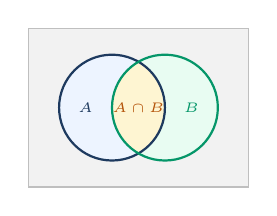
\begin{tikzpicture}[scale=0.56]
            \fill[gray!10] (-2.5,-1.8) rectangle (2.5,1.8);
            \draw[gray!50] (-2.5,-1.8) rectangle (2.5,1.8);
            \fill[lightblue!50] (-0.6,0) circle (1.2cm);
            \fill[lightgreen!50] (0.6,0) circle (1.2cm);
            \begin{scope}
                \clip (-0.6,0) circle (1.2cm);
                \fill[lightamber!80] (0.6,0) circle (1.2cm);
            \end{scope}
            \draw[navyblue, thick] (-0.6,0) circle (1.2cm);
            \draw[codegreen, thick] (0.6,0) circle (1.2cm);
            \node[navyblue, font=\bfseries\tiny] at (-1.2,0) {$A$};
            \node[codegreen, font=\bfseries\tiny] at (1.2,0) {$B$};
            \node[amber, font=\bfseries\tiny] at (0,0) {$A \cap B$};
        \end{tikzpicture}

        \vspace{0.1cm}
        \begin{alertblock}{\scriptsize In C++: popcount}
            \scriptsize \texttt{popcount(a|b)}\\
            $=$ \texttt{popcount(a)} $+$ \texttt{popcount(b)}\\
            $-$ \texttt{popcount(a\&b)}\\[2pt]
            Bitmask Inclusion-Exclusion!
        \end{alertblock}
    \end{columns}
\end{frame}

% ══ BIT REPRESENTATION ═══════════════════════════════════
\begin{frame}[t,shrink=5]{Computer Representation: Bit Strings}
    \small
    \vspace{0.1cm}
    \begin{block}{Idea}
        \footnotesize
        $U = \{a_1, a_2, \ldots, a_n\}$을 순서대로 나열한 뒤,\\
        부분집합 $A$를 길이 $n$의 bit string 으로 표현: $i$-th bit $= 1$ iff $a_i \in A$
    \end{block}

    \vspace{0.1cm}
    \begin{columns}[T]
        \column{0.48\textwidth}
        \textbf{Example: $U = \{1,2,\ldots,10\}$}
        \vspace{0.05cm}

        \scriptsize
        \renewcommand{\arraystretch}{1.2}
        \begin{tabular}{ll}
            \toprule
            \textbf{Set} & \textbf{Bit String} \\
            \midrule
            Odd: $\{1,3,5,7,9\}$ & \texttt{10 1010 1010} \\
            Even: $\{2,4,6,8,10\}$ & \texttt{01 0101 0101} \\
            $\leq 5$: $\{1,2,3,4,5\}$ & \texttt{11 1110 0000} \\
            \bottomrule
        \end{tabular}
        \renewcommand{\arraystretch}{1}

        \vspace{0.1cm}
        \begin{alertblock}{\scriptsize Why Bits?}
            \scriptsize Element listing needs $O(n)$ search for\\
            union/intersection, but bit representation\\
            enables \textbf{hardware-level} single-op processing
        \end{alertblock}

        \column{0.48\textwidth}
        \textbf{Bitwise $=$ Set Operation}
        \vspace{0.05cm}

        \scriptsize
        $A = \{1,2,3,4,5\}$: \texttt{11 1110 0000}\\
        $B = \{1,3,5,7,9\}$: \texttt{10 1010 1010}\\[6pt]
        \textbf{Union} ($A \cup B$):\\
        \texttt{11 1110 0000 $\lor$ 10 1010 1010}\\
        $=$ \texttt{11 1110 1010} $\to$ $\{1,2,3,4,5,7,9\}$\\[4pt]
        \textbf{Intersection} ($A \cap B$):\\
        \texttt{11 1110 0000 $\land$ 10 1010 1010}\\
        $=$ \texttt{10 1010 0000} $\to$ $\{1,3,5\}$\\[4pt]
        \textbf{Complement} ($\overline{A}$):\\
        $\lnot$\texttt{11 1110 0000} $=$ \texttt{00 0001 1111}

        \vspace{0.1cm}
        \begin{exampleblock}{}
            \scriptsize
            \textbf{OR} $\leftrightarrow$ $\cup$ \quad
            \textbf{AND} $\leftrightarrow$ $\cap$\\
            \textbf{NOT} $\leftrightarrow$ $\overline{\phantom{A}}$ \quad
            \textbf{XOR} $\leftrightarrow$ $\oplus$ (symmetric diff.)
        \end{exampleblock}
    \end{columns}
\end{frame}

% ══ C++ SET IMPLEMENTATIONS ══════════════════════════════
\begin{frame}[fragile,shrink=8]{Sets in C++}
    \small
    \begin{columns}[T]
        \column{0.48\textwidth}
        \textbf{Bitmask (single integer)}
\begin{lstlisting}[style=cpp]
// U={1,..,5}, A={1,3,5}, B={1,2,4}
int A = 0b10101; // bit i = elem i
int B = 0b01011;
int U = 0b11111;

int uni  = A | B;  // union
int intr = A & B;  // intersection
int diff = A & ~B; // difference
int comp = U & ~A; // complement
int sym  = A ^ B;  // sym. diff.

// |A| = popcount
int sz = __builtin_popcount(A);

// x in A? (x=3)
bool in = (A >> 3) & 1;
\end{lstlisting}

        \column{0.48\textwidth}
        \textbf{std::set}
\begin{lstlisting}[style=cpp]
#include <set>
set<int> A = {1, 3, 5};
set<int> B = {1, 2, 4};

// insert: A U {7}
A.insert(7);
// erase:  A - {3}
A.erase(3);
// x in A?
bool ok = A.count(5) > 0;
// |A|
int sz = A.size();
\end{lstlisting}

        \vspace{0.05cm}
        \begin{block}{\scriptsize Comparison}
            \scriptsize
            Bitmask: $O(1)$, \; $n \leq 64$\\
            \texttt{bitset<N>}: $O(N/64)$, large $N$\\
            \texttt{std::set}: $O(\log n)$, no size limit
        \end{block}
    \end{columns}
\end{frame}

% ══ MULTISET ═════════════════════════════════════════════
\begin{frame}[t,shrink=3]{Multiset}
    \small
    \vspace{0.1cm}
    \begin{block}{Definition}
        \footnotesize
        \textbf{Multiset}은 원소의 \textbf{중복을 허용}하는 집합입니다.\\
        각 원소가 몇 번 등장하는지(\textbf{multiplicity})가 중요합니다.\\[4pt]
        Notation: $\{a, a, a, b, b\}$ or $\{3 \cdot a,\; 2 \cdot b\}$ \qquad Cardinality: $3 + 2 = 5$
    \end{block}

    \vspace{0.1cm}
    \begin{columns}[T]
        \column{0.48\textwidth}
        \textbf{Multiset Operations}
        \vspace{0.05cm}

        \footnotesize
        $P = \{3 \cdot a, 2 \cdot b\}$, \; $Q = \{1 \cdot a, 4 \cdot b\}$
        \vspace{0.1cm}

        \scriptsize
        \renewcommand{\arraystretch}{1.3}
        \begin{tabular}{ll}
            \toprule
            \textbf{Operation} & \textbf{Result} \\
            \midrule
            $P \cup Q$ (max) & $\{3 \cdot a, 4 \cdot b\}$ \\
            $P \cap Q$ (min) & $\{1 \cdot a, 2 \cdot b\}$ \\
            $P - Q$ & $\{2 \cdot a, 0 \cdot b\}$ \\
            $P + Q$ (sum) & $\{4 \cdot a, 6 \cdot b\}$ \\
            \bottomrule
        \end{tabular}
        \renewcommand{\arraystretch}{1}

        \column{0.48\textwidth}
        \begin{exampleblock}{In C++: \texttt{std::multiset}}
            \scriptsize
\begin{lstlisting}[style=cpp,basicstyle=\ttfamily\tiny\color{codefg}]
#include <set>
multiset<int> ms;
ms.insert(3); ms.insert(3); ms.insert(5);
// ms = {3, 3, 5}

// multiplicity of 3
int cnt = ms.count(3); // 2

// erase one copy
ms.erase(ms.find(3));
// ms = {3, 5}

// erase all copies of 3
ms.erase(3);
\end{lstlisting}
        \end{exampleblock}

        \vspace{0.05cm}
        \begin{alertblock}{\scriptsize REMARK}
            \scriptsize Sorted + duplicates allowed?\\
            $\to$ \texttt{multiset} is the go-to container.
        \end{alertblock}
    \end{columns}
\end{frame}

% ══ COUNTABLE / UNCOUNTABLE ══════════════════════════════
\begin{frame}[t]{Countable vs Uncountable Sets}
    \small
    \vspace{0.1cm}
    \begin{block}{Countable Set}
        \footnotesize
        원소를 $a_1, a_2, a_3, \ldots$ 처럼 자연수와 bijection 시킬 수 있는 집합\\[4pt]
        e.g.\ $\mathbb{N}$, $\mathbb{Z}$, $\mathbb{Q}$ -- all countable
    \end{block}

    \vspace{0.1cm}
    \begin{alertblock}{Uncountable Set}
        \footnotesize
        자연수와 bijection이 \textbf{불가능}한 무한 집합\\[4pt]
        e.g.\ $\mathbb{R}$ -- proved by Cantor's diagonal argument
    \end{alertblock}

    \vspace{0.15cm}
    \begin{exampleblock}{CS Motivation}
        \footnotesize
        \textbf{Programs}의 집합은 countable (source code = finite string)\\
        \textbf{Functions} $\mathbb{N} \to \{0,1\}$의 집합은 uncountable\\[4pt]
        $\Rightarrow$ 프로그램으로 계산할 수 없는 함수가 \textbf{반드시 존재}\\
        $\Rightarrow$ \textbf{Halting Problem}의 undecidability 등\\[4pt]
        이 내용은 Theory of Computation에서 깊이 다루게 됩니다.
    \end{exampleblock}
\end{frame}

% ══════════════════════════════════════════════════════════
% PART 2: FUNCTIONS (Brief)
% ══════════════════════════════════════════════════════════

% ══ FUNCTIONS ════════════════════════════════════════════
\begin{frame}[t,shrink=5]{Functions -- Expressed via Sets}
    \small
    \vspace{0.05cm}
    \begin{block}{Definition}
        \footnotesize
        Function $f: A \to B$ 는 $A$의 각 원소에 $B$의 원소를 \textbf{정확히 하나씩} 대응시키는 규칙\\[3pt]
        수학적으로: $f \subseteq A \times B$, where for each $a \in A$, $\exists!\ b$ s.t.\ $(a, b) \in f$
    \end{block}

    \vspace{0.05cm}
    \begin{columns}[T]
        \column{0.48\textwidth}
        \footnotesize
        $A$: \textbf{domain} \quad $B$: \textbf{codomain}\\
        $f(A) = \{f(a) \mid a \in A\}$: \textbf{range}

        \vspace{0.1cm}
        \textbf{Types of Functions}
        \vspace{0.05cm}
        \scriptsize
        \begin{itemize}\setlength\itemsep{0.15em}
            \item \textbf{Injective (One-to-One)}:\\
                  $f(a) = f(b) \Rightarrow a = b$\\
                  distinct inputs $\to$ distinct outputs
            \item \textbf{Surjective (Onto)}:\\
                  $\forall b \in B,\; \exists a,\; f(a) = b$\\
                  every element in $B$ is mapped to
            \item \textbf{Bijective}: Injective $+$ Surjective\\
                  inverse $f^{-1}$ exists
        \end{itemize}

        \column{0.48\textwidth}
        \centering
        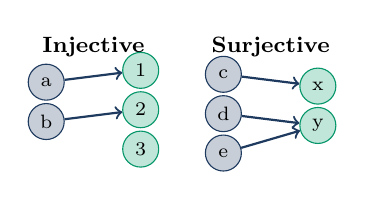
\begin{tikzpicture}[scale=0.5, font=\scriptsize,
            nd/.style={circle, fill=navyblue!25, draw=navyblue, minimum size=13pt, inner sep=0}]
            % Injective
            \node[font=\footnotesize\bfseries] at (0, 3.2) {Injective};
            \foreach \y/\lab in {2.3/a, 1.3/b} {
                \node[nd] (A\lab) at (-1.2, \y) {\lab};
            }
            \foreach \y/\lab in {2.6/1, 1.6/2, 0.6/3} {
                \node[nd, fill=codegreen!25, draw=codegreen] (B\lab) at (1.2, \y) {\lab};
            }
            \draw[->, thick, navyblue] (Aa) -- (B1);
            \draw[->, thick, navyblue] (Ab) -- (B2);

            % Surjective
            \node[font=\footnotesize\bfseries] at (4.5, 3.2) {Surjective};
            \foreach \y/\lab in {2.5/c, 1.5/d, 0.5/e} {
                \node[nd] (C\lab) at (3.3, \y) {\lab};
            }
            \foreach \y/\lab in {2.2/x, 1.2/y} {
                \node[nd, fill=codegreen!25, draw=codegreen] (D\lab) at (5.7, \y) {\lab};
            }
            \draw[->, thick, navyblue] (Cc) -- (Dx);
            \draw[->, thick, navyblue] (Cd) -- (Dy);
            \draw[->, thick, navyblue] (Ce) -- (Dy);
        \end{tikzpicture}

        \vspace{0.08cm}
        \begin{alertblock}{\scriptsize REMARK}
            \scriptsize
            \textbf{Injective}: collision-free hash function\\
            \textbf{Bijective}: encryption ($f^{-1}$ = decryption)\\
            In C++: \texttt{std::map<A,B>} = mapping\\[2pt]
        \end{alertblock}
    \end{columns}
\end{frame}

% ══════════════════════════════════════════════════════════
% PART 3: MATRICES
% ══════════════════════════════════════════════════════════

% ══ MATRIX DEFINITION ════════════════════════════════════
\begin{frame}[t,shrink=3]{Matrix -- Definition}
    \small
    \vspace{0.1cm}
    \begin{block}{Definition}
        \textbf{Matrix}는 수를 직사각형으로 배열한 구조입니다.\\[3pt]
        \footnotesize $m \times n$ matrix: $m$ rows, $n$ columns, \; entry $a_{ij}$: row $i$, column $j$\\[3pt]
        Two matrices are equal iff same size and all corresponding entries are equal.
    \end{block}

    \vspace{0.1cm}
    \begin{columns}[T]
        \column{0.48\textwidth}
        \textbf{Basic Operations}
        \vspace{0.05cm}

        \footnotesize
        \textbf{Addition}: same size, entry-wise\\[3pt]
        $\begin{bmatrix} 1 & 2 \\ 3 & 4 \end{bmatrix} + \begin{bmatrix} 0 & 1 \\ 2 & 1 \end{bmatrix} = \begin{bmatrix} 1 & 3 \\ 5 & 5 \end{bmatrix}$

        \vspace{0.15cm}
        \textbf{Multiplication}: $A$ ($m \times k$), $B$ ($k \times n$) $\to$ $AB$ ($m \times n$)\\[3pt]
        $(AB)_{ij} = \displaystyle\sum_{l=1}^{k} a_{il} \cdot b_{lj}$

        \vspace{0.1cm}
        $\begin{bmatrix}1&2\\3&4\end{bmatrix}\begin{bmatrix}0&1\\2&1\end{bmatrix} = \begin{bmatrix}4&3\\8&7\end{bmatrix}$

        \column{0.48\textwidth}
        \textbf{Special Matrices}
        \vspace{0.05cm}

        \footnotesize
        \begin{itemize}\setlength\itemsep{0.2em}
            \item \textbf{Square}: $m = n$
            \item \textbf{Identity} $I_n$: diagonal 1, rest 0\\
                  $AI_n = I_m A = A$
            \item \textbf{Transpose} $A^T$: row $\leftrightarrow$ column\\
                  $(A^T)_{ij} = a_{ji}$
            \item \textbf{Symmetric}: $A = A^T$
        \end{itemize}

        \vspace{0.1cm}
        \begin{alertblock}{REMARK}
            \scriptsize Matrix multiplication is\\
            \textbf{NOT commutative}: $AB \neq BA$ in general
        \end{alertblock}
    \end{columns}
\end{frame}

% ══ MATRIX NON-COMMUTATIVITY EXAMPLE ═════════════════════
\begin{frame}[t]{Matrix Multiplication (Cont.)}
    \small
    \vspace{0.1cm}
    \begin{block}{$AB \neq BA$ -- Example}
        \footnotesize
        $A = \begin{bmatrix}1&2\\3&4\end{bmatrix}$, \quad
        $B = \begin{bmatrix}0&1\\2&1\end{bmatrix}$

        \vspace{0.15cm}
        $AB = \begin{bmatrix}1 \cdot 0 + 2 \cdot 2 & 1 \cdot 1 + 2 \cdot 1\\3 \cdot 0 + 4 \cdot 2 & 3 \cdot 1 + 4 \cdot 1\end{bmatrix} = \begin{bmatrix}4&3\\8&7\end{bmatrix}$

        \vspace{0.1cm}
        $BA = \begin{bmatrix}0 \cdot 1 + 1 \cdot 3 & 0 \cdot 2 + 1 \cdot 4\\2 \cdot 1 + 1 \cdot 3 & 2 \cdot 2 + 1 \cdot 4\end{bmatrix} = \begin{bmatrix}3&4\\5&8\end{bmatrix}$

        \vspace{0.1cm}
        $AB \neq BA$ \quad \checkmark
    \end{block}

    \vspace{0.15cm}
    \begin{exampleblock}{Why Matrices Matter in CS}
        \footnotesize
        \renewcommand{\arraystretch}{1.3}
        \begin{tabular}{ll}
            \textbf{Graph Theory} & Adjacency matrix -- vertex connectivity \\
            \textbf{Database} & Relation matrix -- table correspondence \\
            \textbf{Computer Graphics} & Transformation matrix -- rotation, scaling \\
            \textbf{PS / Competitive} & Boolean matrix product -- path existence \\
            \textbf{Machine Learning} & Weight matrix -- neural network computation \\
        \end{tabular}
        \renewcommand{\arraystretch}{1}
    \end{exampleblock}
\end{frame}

% ══ BOOLEAN MATRIX ═══════════════════════════════════════
\begin{frame}[t,shrink=6]{Boolean Matrix (Zero-One Matrix)}
    \small
    \vspace{0.05cm}
    \begin{block}{Definition}
        \footnotesize 원소가 오직 \textbf{0 또는 1}인 행렬. Set, Relation, Graph를 행렬로 표현할 때 핵심 도구입니다.
    \end{block}

    \vspace{0.08cm}
    \begin{columns}[T]
        \column{0.52\textwidth}
        \textbf{Boolean Operations}
        \vspace{0.05cm}

        \footnotesize
        \begin{itemize}\setlength\itemsep{0.15em}
            \item \textbf{Join} ($A \lor B$): $c_{ij} = a_{ij} \lor b_{ij}$ \; (OR)
            \item \textbf{Meet} ($A \land B$): $c_{ij} = a_{ij} \land b_{ij}$ \; (AND)
            \item \textbf{Boolean Product} ($A \odot B$):\\[2pt]
                  $c_{ij} = \displaystyle\bigvee_{k=1}^{p}(a_{ik} \land b_{kj})$\\[4pt]
                  normal product: $+ \to$ OR, $\times \to$ AND
        \end{itemize}

        \vspace{0.08cm}
        \begin{exampleblock}{\scriptsize Boolean Product Example}
            \scriptsize
            $A = \begin{bmatrix}1&0\\0&1\end{bmatrix}$,\;
            $B = \begin{bmatrix}1&1\\0&1\end{bmatrix}$\\[3pt]
            $A \odot B = \begin{bmatrix}(1{\land}1){\lor}(0{\land}0) & (1{\land}1){\lor}(0{\land}1)\\(0{\land}1){\lor}(1{\land}0) & (0{\land}1){\lor}(1{\land}1)\end{bmatrix} = \begin{bmatrix}1&1\\0&1\end{bmatrix}$
        \end{exampleblock}

        \column{0.44\textwidth}
        \textbf{Adjacency Matrix}
        \vspace{0.05cm}

        \centering
        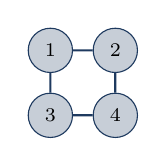
\begin{tikzpicture}[scale=0.55, font=\scriptsize,
            node/.style={circle, fill=navyblue!25, draw=navyblue, minimum size=16pt}]
            \node[node] (1) at (0,1.5) {1};
            \node[node] (2) at (1.5,1.5) {2};
            \node[node] (3) at (0,0) {3};
            \node[node] (4) at (1.5,0) {4};
            \draw[thick, navyblue] (1)--(2) (1)--(3) (2)--(4) (3)--(4);
        \end{tikzpicture}

        \vspace{0.05cm}
        \footnotesize
        $M_G = \begin{bmatrix}0&1&1&0\\1&0&0&1\\1&0&0&1\\0&1&1&0\end{bmatrix}$

        \vspace{0.08cm}
        \begin{alertblock}{\scriptsize REMARK}
            \scriptsize $M_G^{[2]} = M_G \odot M_G$: $(i,j)$ entry $= 1$\\
            $\Leftrightarrow$ path of length 2 from $i$ to $j$ exists\\[2pt]
            $M_G^{[r]}$: path of length $\leq r$
        \end{alertblock}
    \end{columns}
\end{frame}

% ══ BOOLEAN MATRIX C++ ═══════════════════════════════════
\begin{frame}[fragile,shrink=8]{Boolean Matrix in C++}
    \small
    \begin{columns}[T]
        \column{0.5\textwidth}
        \textbf{bitset adjacency matrix}
\begin{lstlisting}[style=cpp]
#include <bitset>
const int N = 4;

// adj[i]: neighbor set of vertex i
bitset<N> adj[N];

void addEdge(int u, int v) {
    adj[u].set(v);
    adj[v].set(u); // undirected
}

// Boolean product: M^[2]
// M2[i][j]=1: path i->k->j exists
bitset<N> M2[N];
for (int i = 0; i < N; i++)
    for (int k = 0; k < N; k++)
        if (adj[i].test(k))
            M2[i] |= adj[k];
\end{lstlisting}

        \column{0.46\textwidth}
        \textbf{Relation as Matrix}
\begin{lstlisting}[style=cpp]
// R in A x B
// A={0,1,2}, B={0,1,2,3}
// R={(0,1),(1,2),(2,0),(2,3)}

bitset<4> R[3];
R[0].set(1); // (0,1)
R[1].set(2); // (1,2)
R[2].set(0); // (2,0)
R[2].set(3); // (2,3)

// Matrix:
// [0 1 0 0]
// [0 0 1 0]
// [1 0 0 1]

// Transitive closure: R^+
// -> Floyd-Warshall with bitset
\end{lstlisting}

        \begin{block}{\scriptsize Performance}
            \scriptsize \texttt{bitset} Boolean matrix product:\\
            $O(n^3)$ $\to$ $O(n^3 / 64)$ (\textbf{64x} speedup)
        \end{block}
    \end{columns}
\end{frame}

% ══ TRANSITIVE CLOSURE ═══════════════════════════════════
\begin{frame}[fragile,shrink=5]{Application: Transitive Closure}
    \small
    \vspace{0.1cm}
    \begin{block}{Idea}
        \footnotesize
        Relation $R$의 \textbf{transitive closure} $R^+$: 간접 도달 가능한 모든 쌍을 추가\\[3pt]
        $(a,b) \in R$ and $(b,c) \in R$ $\Rightarrow$ $(a,c) \in R^+$ \quad (formal definition in Week 3)
    \end{block}

    \vspace{0.08cm}
    \begin{columns}[T]
        \column{0.5\textwidth}
        \textbf{Floyd-Warshall + bitset}
\begin{lstlisting}[style=cpp]
const int N = 500;
bitset<N> reach[N]; // reach[i][j]=1
                    // if i can reach j
// Initialize with direct edges
for (auto [u,v] : edges)
    reach[u].set(v);

// Transitive closure
for (int k = 0; k < N; k++)
    for (int i = 0; i < N; i++)
        if (reach[i].test(k))
            reach[i] |= reach[k];

// Now reach[i][j]=1 iff path i->j
\end{lstlisting}

        \column{0.46\textwidth}
        \begin{exampleblock}{Intuition}
            \footnotesize
            $k$를 경유지로 삼아:\\
            ``$i$에서 $k$로 갈 수 있고,\\
            $k$에서 $j$로 갈 수 있으면,\\
            $i$에서 $j$로 갈 수 있다''\\[6pt]
            This is Boolean matrix product:\\
            \texttt{reach[i] |= reach[k]}\\
            ($i$의 도달 집합에 $k$의 도달 집합을 합침)
        \end{exampleblock}

        \vspace{0.1cm}
        \begin{alertblock}{\scriptsize Complexity}
            \scriptsize $O(N^3 / 64)$ with bitset\\
            $N = 500 \to$ about $2 \times 10^6$ ops
        \end{alertblock}
    \end{columns}
\end{frame}

% ══ RELATIONS PREVIEW ════════════════════════════════════
\begin{frame}[t,shrink=5]{Week 3 Preview: Relations \& Functions}
    \small
    \vspace{0.1cm}
    \begin{block}{This Week's Tools $\to$ Next Week}
        \footnotesize
        $A \times B$ (Cartesian Product) $\to$ Relation $R \subseteq A \times B$\\
        Boolean Matrix $\to$ Matrix representation $M_R$\\
        Function $f: A \to B$ $\to$ Special case of Relation
    \end{block}

    \vspace{0.08cm}
    \begin{columns}[T]
        \column{0.48\textwidth}
        \textbf{Week 3 Topics}
        \vspace{0.03cm}

        \footnotesize
        \renewcommand{\arraystretch}{1.2}
        \begin{tabular}{ll}
            \toprule
            \textbf{Concept} & \textbf{Property} \\
            \midrule
            Reflexive & $\forall a,\; (a,a) \in R$ \\
            Symmetric & $(a,b) \in R \Rightarrow (b,a) \in R$ \\
            Transitive & $(a,b),(b,c) \in R \Rightarrow (a,c) \in R$ \\
            \midrule
            Equivalence & Refl.\ $+$ Sym.\ $+$ Trans. \\
            Partial Order & Refl.\ $+$ Antisym.\ $+$ Trans. \\
            \bottomrule
        \end{tabular}
        \renewcommand{\arraystretch}{1}

        \column{0.48\textwidth}
        \begin{exampleblock}{Example}
            \footnotesize
            $A = \{1,2,3\}$, relation: ``$a \leq b$''\\[3pt]
            $R = \{(1,1),(1,2),(1,3),$\\
            $\phantom{R = \{}(2,2),(2,3),(3,3)\}$\\[3pt]
            $M_R = \begin{bmatrix}1&1&1\\0&1&1\\0&0&1\end{bmatrix}$
        \end{exampleblock}

        \vspace{0.05cm}
        \begin{alertblock}{\scriptsize REMARK}
            \scriptsize Boolean product of $M_R$ computes\\
            Transitive Closure\\
            $\to$ direct application of today's topic!
        \end{alertblock}
    \end{columns}
\end{frame}

% ══ PRACTICE TRACK ═══════════════════════════════════════
\begin{frame}[t,shrink=5]{Practice Track}
    \small
    \vspace{0.1cm}

    \begin{exampleblock}{Basic Track -- BOJ Step 49: Set \& Map (9 problems)}
        \footnotesize
        \renewcommand{\arraystretch}{1.2}
        \begin{tabular}{lll}
            \toprule
            \textbf{\#} & \textbf{Problem} & \textbf{Key Concept} \\
            \midrule
            10815 & Numeric Cards & \texttt{set} -- membership test ($x \in A$?) \\
            14425 & String Set & \texttt{set<string>} -- string membership \\
            7785 & People in Office & \texttt{set} -- insert \& erase \\
            1620 & Pok\'{e}mon Master & \texttt{map} -- bidirectional mapping \\
            10816 & Numeric Cards 2 & \texttt{map} / \texttt{multiset} -- counting \\
            1764 & Never Seen Never Heard & \texttt{set} -- intersection ($A \cap B$) \\
            1269 & Symmetric Difference & \texttt{set} -- $A \oplus B = (A-B) \cup (B-A)$ \\
            11478 & Distinct Substrings & \texttt{set} -- duplicate removal \\
            11403 &경로 찾기 & \texttt{Matrix} -- boolean Matrix \\ 
            \bottomrule
        \end{tabular}
        \renewcommand{\arraystretch}{1}
    \end{exampleblock}

    \vspace{0.08cm}
    \begin{alertblock}{REMARK}
        \footnotesize
        오늘 배운 집합 이론이 그대로 STL설계에 반영되어 있습니다.\\
        \texttt{set}, \texttt{map}, \texttt{multiset} 등 STL container를 자유롭게 활용해보세요.
    \end{alertblock}
\end{frame}

% ══ PRACTICE TRACK (Cont.) ═══════════════════════════════
\begin{frame}[t]{Practice Track (Cont.)}
    \small
    \vspace{0.2cm}

    \begin{block}{Advanced Track -- BOJ 1717: Disjoint Set (Union-Find)}
        \footnotesize
        \textbf{Link}: \texttt{acmicpc.net/problem/1717}\\[4pt]
        \textbf{Goal}: 집합의 합치기(union)와 같은 집합 판별(find) 구현\\[4pt]
        \textbf{Hint}: ``$a$와 $b$가 같은 집합에 속하는가?'' $\to$ Union-Find (Disjoint Set)\\
        Path compression $+$ union by rank 으로 amortized $O(\alpha(n))$\\[4pt]
        \textbf{Connection}: 집합의 partition 과 equivalence relation (Week 3 preview)
    \end{block}

    \vspace{0.15cm}
    \begin{alertblock}{Challenge Track -- BOJ 22940: Linear System of Equations}
        \footnotesize
        \textbf{Link}: \texttt{acmicpc.net/problem/22940}\\[4pt]
        \textbf{Goal}: 행렬 연산을 이용한 연립 방정식 풀기\\[4pt]
        \textbf{Hint}: $n$차 연립 방정식을 $AX = B$ 형태의 행렬 곱으로 표현한 뒤,\\
        Gaussian Elimination 으로 해를 구합니다.\\[4pt]
        \textbf{Connection}: 오늘 배운 행렬 곱의 직접적 활용!
    \end{alertblock}

    \vspace{0.15cm}
    
\end{frame}

% ══ WEEK 3 ROADMAP ═══════════════════════════════════════
\begin{frame}[t,shrink=3]{Summary \& Week 3 Preview}
    \vspace{0.2cm}
    \begin{columns}[T]
        \column{0.3\textwidth}
        \begin{block}{\footnotesize Week 1}
            \footnotesize \textbf{Propositions \& Logic}
            \vspace{0.1cm}

            \centering
            \small $p \land q$\\$p \lor q$\\$p \rightarrow q$
            \vspace{0.1cm}

            \footnotesize\textit{Logic, SAT}
        \end{block}

        \column{0.3\textwidth}
        \begin{exampleblock}{\footnotesize Week 2 -- Today}
            \footnotesize \textbf{Sets \& Matrices}
            \vspace{0.1cm}

            \centering
            \small $A \cap B$\\$A \cup B$\\$M_R$
            \vspace{0.1cm}

            \footnotesize\textit{Sets, Matrix}
        \end{exampleblock}

        \column{0.3\textwidth}
        \begin{block}{\footnotesize Week 3}
            \footnotesize \textbf{Relations \& Functions}
            \vspace{0.1cm}

            \centering
            \small $R \subseteq A{\times}B$\\$f: A \to B$\\$R^+$
            \vspace{0.1cm}

            \footnotesize\textit{Relations, Functions}
        \end{block}
    \end{columns}

    \vspace{0.3cm}
    \begin{center}
    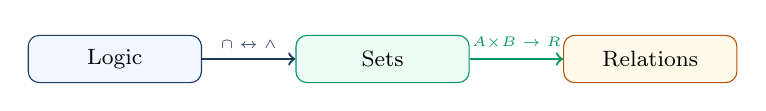
\begin{tikzpicture}[scale=0.85, font=\footnotesize]
        \node[draw=navyblue, fill=lightblue!40, rounded corners, minimum width=2.2cm, minimum height=0.6cm] (w1) at (0,0) {Logic};
        \node[draw=codegreen, fill=lightgreen!40, rounded corners, minimum width=2.2cm, minimum height=0.6cm] (w2) at (4,0) {Sets};
        \node[draw=amber, fill=lightamber!40, rounded corners, minimum width=2.2cm, minimum height=0.6cm] (w3) at (8,0) {Relations};
        \draw[->, thick, navyblue] (w1) -- node[above, font=\tiny] {$\cap\leftrightarrow\land$} (w2);
        \draw[->, thick, codegreen] (w2) -- node[above, font=\tiny] {$A{\times}B \to R$} (w3);
    \end{tikzpicture}
    \end{center}

\end{frame}

\end{document}